\documentclass{samkoelleprelimworking}
%%\setlength{\oddsidemargin}{0.25in} %%\setlength{\textwidth}{6in} %%\setlength{\topmargin}{0.5in} %%\setlength{\textheight}{9in}
\usepackage{amsmath}
\usepackage{url}
\usepackage{epstopdf,gensymb}
\usepackage{graphics}
\usepackage{graphicx}
%\usepackage[numbers]{natbib}
%\usepackage{endfloat}
\usepackage{amsfonts, animate,subfigure}
\usepackage{amsthm,amsmath,amssymb}
%%\usepackage[margin=1in]{geometry}
\usepackage{bbm}
%\usepackage[sc]{mathpazo}
%\linespread{1.05}  
\usepackage{setspace}
\usepackage[export]{adjustbox}
\usepackage{amsmath}
\usepackage{bm}
\usepackage[normalem]{ulem}
\usepackage{mathtools}
\usepackage{wrapfig}
\usepackage[usenames,dvipsnames]{xcolor}
\usepackage[section]{placeins}

\usepackage{mathrsfs}

\usepackage{thmtools}

\setlength{\textfloatsep}{10pt plus 1.0pt minus 2.0pt}
\renewcommand{\baselinestretch}{1.5}
\bibliographystyle{plainnat}
\renewcommand{\d}[1]{\mathbb{#1}}
\DeclareMathOperator{\sgn}{sgn}
\DeclareMathOperator\erf{erf}
\DeclareMathOperator*{\argmin}{arg\,min}
\setlength{\belowcaptionskip}{2pt plus 0pt minus 0pt}
\newcommand{\defeq}{\vcentcolon=}
\newcommand{\eqdef}{=\vcentcolon}
\newcommand{\vmdel}[1]{\sout{#1}}
\newcommand{\me}{\mathrm{e}}
\newcommand{\vmadd}[1]{\textbf{\color{red}{#1}}}
\newcommand{\vmcomment}[1]{({\color{blue}{VM's comment:}} \textbf{\color{blue}{#1}})}
\newcommand{\skcomment}[1]{({\color{purple}{SK's comment:}} \textbf{\color{purple}{#1}})}
\begin{document} %%\maketitle
\begin{center}  
{\LARGE Square Root Graphical Models: Multivariate Generalizations of
Univariate Exponential Families that Permit Positive Dependencies, by David Inouye, Pradeep Ravikumar, and Inderjit Dhillon}\\\ \\   
 {Samson Koelle \\
    Department of Statistics, University of Washington Seattle, WA, 98195, USA  
     } 
  \end{center}
  
\begin{abstract} 
 
%\section{Abstract}

Understanding relationships between different categorical or quantitative random variables is a central problem in clustering, network reconstruction, and regression.  This paper proposes a multivariate distribution based on a Markov Random Field which encapsulates multivariate Gaussian and Ising graphical models.  The parameter space is expanded using a square root transformation of sufficient statistics to enable new multivariate dependencies.
\end{abstract}

\section{Introduction} 

Discovery of positive and negative tendencies to co-occur between empirical random variables is an important motivation for fitting multivariate distributions to data.  For this reason, Markov Random Fields (MRFs), which specify conditional dependencies between random variables, are often used to model multivariate data.  The commonly used multivariate Gaussian and Ising distributions are examples of Markov Random Fields, and the learning of MRF model structures, particularly when the number of variables is high, is an active area of research.

Despite the numerous established tools for fitting multivariate Gaussian distributions, alternative multivariate distributions are somewhat lacking.  In practice, data is often transformed to be Gaussian, and methods developed for multivariate Gaussians are often applied to data which is not Gaussian.  This can be problematic.  For example, exponential and Poisson random variables have different asymptotic tail behavior than Gaussians.  This discrepancy can harm model optimization given rare events.  A somewhat related option is the use of a Gaussian copula, in which latent variables leading to non-Gaussian observables are themselves assumed to be distributed \vmadd{as} multivariate Gaussian.  However, the imposition of a copula structure may be unfounded, and copulas also require more data to optimize than methods in which Gaussian and non-Gaussian distributions don't have to simultaneously inferred.  Non-parametric methods also increase the quantity of data required for a given power of inference.  The impetus to Gaussianize is also driven by insufficiencies of the multivariate exponential and Poisson distributions.   The multivariate exponential distribution has a singular region with high probability mass, and the multivariate Poisson distribution can only model random variables with a positive tendency to co-occur.  Even the underlying assumption of these models, that the presence of a latent univariate Poisson or exponential random variables corresponds to dependencies between pairs of observed variables, is not always applicable. 

The alternative approach of this paper is that the parameters of univariate distributions are functions of effector variables.  The question that it tries to answer is what form are these functions allowed to take, in order that the joint distribution of effectors and effectees is a Markov Random Field?  The \textit{Square Root Graphical Model} (SRM) results from the relaxation of a previous assumption that conditional distributions are from a specified univariate exponential family distribution, which we call the base family.  We still insist that all univariate conditionals have tail behavior and domain from the base family, and that independent random variables have the option of being from this base family.  Taking square roots of univariate sufficient statistics ensures the the terms with the largest asymptotic growth in the joint distribution are of the same order as the terms with the largest growth in the base exponential family.  Using this fact, multivariate tail behavior is shown to be normalizable under weak conditions.  In contrast with a previous MRF model, positive dependencies between both Poisson and exponential random variables do not interfere with normalization. This is illustrated by fitting an SRM on a dataset of airport delay times using standard methods.  The normalizing constant is approximated to allow \vmadd{for} model comparison.

\vmcomment{I hope that when you add references, the story of what has been done in the past will become more clear. Also, would be nice to have examples of MRF usage to solve concrete problems.}

\section{Methods}

In this section, I describe the derivation of the SRM distribution, the properties which lead to its normalizability, its fitting using proximal gradient descent, and the stochastic approximation of its normalizing constant.  We are given data $\mathbb{X}$ composed of a set of $n$ observations of $p$ variables $\bm{x} = \{x_1, \dotsc , x_p\}$.  $\bm{x}_{-s} \vcentcolon = \bm{x} \setminus x_s$. Generally, vectors will be bolded, and matrices capitalized.

 \subsection{Graphical Models}
 
A graph $\bm{G}$ consists of a set of nodes or vertices $\bm{V} = \{V_1, \dotsc , V_p \}$ and a set of edges $\bm{E}$ which link the nodes in a pairwise manner.  Self-edges are allowed.  Given a multivariate vector of univariate random variables $\bm{x}$ which takes values in a domain $\mathcal{D}$ and is bijected with $V$ \vmcomment{Not sure I know what it means ``to be bijected with something''}, define a Markov Random Field probability measure $P(\bm{x})$ as satisfying the following properties.
\begin{enumerate}
\item $P(\bm{x}) > 0 \; \forall \bm{x} \in \mathcal{D}$
\item $P(x_s \vert \bm{x}_{-s}) = P(x_s \vert \bm{x}_{-s,-t})$ implies $e_{st} \not\in E$, where $\bm{x}_{-s,-t}$ is the multivariate random vector $\bm{x}$ with the s-th and t-th entries removed and $e_{st}$ is an edge linking the nodes corresponding to $x_s$ and $x_t$.
\item $P(x_s \vert \bm{x}_{-s}) = P(x_s \vert \bm{N}(x_s))$, where $ \bm{N}(x_s)$ denotes the set of univariate random variables whose corresponding nodes are connected to the node of $x_s$ via an edge. 
\item $P(\bm{x}_A \vert \bm{x}_{B \cap C}) = P(\bm{x}_A \vert \bm{x}_C)$, where $A$, $B$, and $C$ are non-intersecting sets of nodes, and every path from $A$ to $B$ in $\bm{E}$ passes through $C$.
\end{enumerate}
MRFs are flexible.  Nodes may correspond to either latent factors or observables, and edges may be of quantitatively different strengths, though they are also binary in the Markov sense \vmcomment{Edges are just binary, there is no need for ``Markov sense''.}.  While the above conditions make no restriction on the minimality of the edge set $\bm{E}$, they also enable removal of edges between variables which are independent conditionally on interpolating paths in the graph.  Since it is not always obvious which conditional probability dependencies are spurious given others, and since non-spurious edges are potentially indicative of interesting causal links or latent factors, we will optimize our MRF using a penalty in \ref{optimization}

The Hammersley-Clifford Theorem implies that the density of a multivariate probability measure of a Markov Random Field such as the one described in the previous paragraph factors as
 \[P (\bm{x}) = \frac{1}{Z(\Phi)} \exp \sum_{c \in \mathcal{C}}\phi_c(\bm{x}).\]
The \textit{cliques} $\mathcal{C}$ are simplicial combinations of edges in the base graph, and the \textit{clique-specific compatibility functions} $\phi_c$ only on the variables whose nodes are in the clique.  The \textit{normalizing constant} $Z(\Phi)$ depends on the set of compatibility functions $\Phi = \{\phi_c \vert c \in \mathcal{C} \}$ as well as the domain of $\bm{x}$, and ensures that the distribution integrates to $1$.  The theorem states that assignment of random variables to nodes and conditional probability dependencies to edges is equivalent to the choices of compatibility functions corresponding to conditional probability simplices, given the domain $\mathcal{D}$ of our probability measure.  Note that these choices are constrained by the necessary condition that 
\[Z(\Phi) = \int_\mathcal{D} \exp \sum_{c \in \mathcal{C}}\phi_c(\bm{x}) d\bm{x} < \infty,\]
i.e. that the distribution is \textit{normalizable}.  The next section introduces some background on univariate distributions which will inform our choices of compatibility functions.
 
\subsection{Exponential Family Distributions}

The exponential family of distributions for a univariate random variable $x$ includes all probability laws of the form
  \[P(x|\theta) = \exp(\eta(\theta)^T T(x) + B(x) - A(\theta)),\]
  where $\eta(\theta)$ are the \textit{natural parameters} of the exponential family, $T(x)$ is a set of \textit{sufficient statistics}, $B(x)$ is the \textit{base measure} of the distribution, and 
  \[A(\theta) = \log \int_{\mathcal{D}} \exp(\eta(\theta)^T T(x) + B(x))dx\]
  is the \textit{normalizing constant}.   This class includes many commonly encountered discrete and continuous distributions, several of which are summarized in the table below.

\begin{center}
\begin{table}[h!]
\resizebox{\textwidth}{!}{
    \begin{tabular}{| l | l | l | l | l | l |}
    \hline
    Name & Standard PDF & $\eta ( \theta)$ & $T(x)$ & $B(x)$ & $A(\theta)$ \\ \hline
    Bernoulli & $p^x (1-p)^x$ & $\log (\frac{p}{1-p})$ & $x$ & $0$ & $-\log (1-p)$ \\ \hline
    Exponential & $\lambda \me^{- \lambda x}$ & $-\lambda$ & $x$ & $0$ & $-\log \lambda $ \\ \hline
    Poisson & $\frac{\lambda^x \me^{- \lambda}}{x!}$ & $-\log \lambda$ & $x$ & $-\log x!$ & $\lambda$ \\ \hline
    Normal & $\frac{1}{\sigma \sqrt{2 \pi}} \exp{\frac{-(x-\mu)^2}{2\sigma^2}}$ & $\{\frac{\mu}{\sigma^2}, \frac{-1}{2 \sigma^2} \}$ & $\{x, x^2 \}$ & $-\frac{1}{2} \log (2 \pi)$ & $\frac{\mu^2}{2\sigma^2} + \log{\sigma} $ \\ \hline
    Multivariate Normal & $\frac{1}{\sqrt{{(2 \pi)}^p | \Sigma |}} \exp{\frac{-(\bm{x}-\bm{\mu})^T \Sigma^{-1} (\bm{x}-\bm{\mu})}{2}}$ & $\{\Sigma^{-1} \mu, \frac{-1}{2} \Sigma^{-1} \}$& $\{\bm{x}, \bm{x}^T \bm{x} \}$ & $\frac{-p}{2} \log (2\pi)$& $\frac{\bm{\mu}^T \Sigma^{-1} \bm{\mu}}{2} + \frac{\log | \Sigma |}{2}$\\
    \hline
    \end{tabular}}
    \caption{Exponential family parameterizations of selected distributions.}
    \end{table}
\end{center}

The prevalence of exponential family distributions in univariate statistics is based upon a number of useful properties, including that $T(\{x_1, \dotsc x_n\}) = \sum_{i=1}^n T(x_i)$, a set of fixed size, is sufficient for maximum likelihood optimization of the model given arbitrarily large numbers of observations.  This follows immediately from the product law $P(\{x_1, \dotsc x_n\}) = \prod_{i = 1}^n P(x_i)$ and the fact that the data and parameters only interact in the first term of the exponential.  Furthermore, exponential family distributions are maximum entropy distributions given given its domain and certain constraints on moments.  For example, the univariate normal distribution is the maximum entropy distribution over the reals with specified first and second moments. Because of this maximum entropy characterization, exponential family distributions appear both in physical and information theoretic systems, and are useful as minimally informative priors.
  
\subsection{Exponential Family Markov Random Fields}

For the above reasons, we often wish to model a particular variable with a univariate exponential family distribution.  Let us assume that the conditional probability distribution of each random variable in our MRF given all others is from a univariate exponential family, and thus that the natural parameter $\eta$ is in fact a function of these effector variables, i.e.
\begin{align}
P(x_s \vert \bm{x}_{-s}) = \exp(\eta(\bm{x_{-s}}) T(x_s) + B(x_s) - A_s), 
\end{align}
where $A_s$ is the normalizing constant of this conditional distribution.  As shown in \citep{Besag1974-qb} and \citep{Yang2013-wa}, in order for 1) univariate conditionals to be of this form and 2) the joint distribution to be an MRF, the functions $\eta (x_{-s})$ must be of the form
\[\eta (\bm{x}_{-s}) = \sum_{c \in \mathcal{C}_s} (\theta_c \prod_{t \in c \setminus s } T(x_t) )   ,\]
where $\mathcal{C}_s$ is the set of cliques containing site $s$, $\theta_c \in \Theta_{\mathcal{C}_s}$ are clique-specific scalar parameters, $B(x_s)$ is the base measure of the univariate exponential family of node $s$.  These conditionals specify a joint distribution of the form \[P(\bm{x}) = \exp(\sum_{s=1}^p (\eta(\bm{x_{-s}}) T(x_s) + B(x_s)) - A).\]
This theorem states that in order for a MRF to have node-conditional distributions from an exponential family, its compatibility functions must be equivalent to a scalar clique weights multiplied by the sufficient statistics of the variables in the clique, i.e.
\[\phi_c = \theta_c \prod_{s \in c} T(x_s)\]
Though this constraint may seem surprising given the general lack of restriction on compatibility functions, remember that $\theta_c$ and $T(x)$ are allowed to be vectors.  This will provide one way of instantiating a multivariate Gaussian (which has sufficient statistics $\{x, x^2\}$ using the above joint distribution.

Rewriting the joint distribution
\begin{align}
 P(\bm{x} \vert \Theta) &= \exp{ (\sum_{s=1}^p ( \sum_{c \in \mathcal{C}_s} (\theta_c \prod_{t \in c} T(x_t) ) + B(x_s)) - A(\Theta ))}.
 \end{align}
 and considering only pairwise graphical models, whose cliques of order $> 2$ we ignore, the resultant probability law is
 \begin{align}
  P(\bm{x} \vert \Theta,\Phi) &= \exp(\Theta^{T} T(\bm{x}) + T(\bm{x})^T\Phi  T(\bm{x}) + \sum_{s=1}^p B(x_s) - A(\Theta, \Phi)) \\
  &= \exp(\Theta^{T} T(\bm{x}) + T(\bm{x})^T\Phi  T(\bm{x}) + \bm{B}(\bm{x}) - A(\Theta, \Phi))
  \end{align}
 where $\bm{B}(\bm{x})  \vcentcolon = \sum_{s=1}^p B(x_s)$ and $\Theta \in \mathbb{R}^p$ and $\Phi \in \mathbb{R}^{p\times p}$ are clique-specific parameters of orders $1$ and $2$ respectively. By the theorem stated above, these arrays completely specify the underlying compatibility functions.  Recall that each node is trivially a univariate clique, and by the earlier assumption that self-edges exist, the diagonals of $\Phi$ are not required to be zero.   However, the node conditionals of this MRF are 
 \begin{align}
 P(x_s \vert \bm{x}_{-s}) &= \exp ( \Theta_s T(x_s) + 2 T(\bm{x_{-s}})^T \Phi_{-s} T(x_s) + \Phi_{ss} {T(x_s)}^2 + B(x_s) - A_s) \\
 \end{align}
and so they often must be zero in order for the conditionals to have tails from the base family.  This imposes the further limitation that for MRFs with univariate conditionals from an exponential family with $T(x) = x$, $\Phi_{st} \leq 0 \; \forall \; s \neq t$.   Note that this limitation on diagonals does not apply to the multivariate Gaussian distribution, which has quadratic tails.  The joint density of the multivariate Gaussian distribution described by the natural parameterization $\Theta = \Sigma^{-1} \mu$ and $\Phi = -\frac{1}{2}\Sigma^{-1}$, $\bm{B}(\bm{x}) = {(2 \pi )} ^{\frac{-k}{2}}$, $T(\bm{x}) = \bm{x}$, and an appropriate normalizing constant.   \citep{Besag1974-qb} and \citep{Yang2013-wa} provide slightly alternative parameterizations.   In both cases, variance is assumed to be known, and is included in the base measure, though \citep{Besag1974-qb} sets the diagonals of $\Phi \vcentcolon \Phi_{\text{diag}} = \bm{1}$ and \citep{Yang2013-wa} $= \bm{0}$.  Generally, incorporating parameters into the base measure precludes optimization using sufficient statistics.  

\subsection{Square Root Graphical Models}
\begin{figure}\label{fig:expdists}
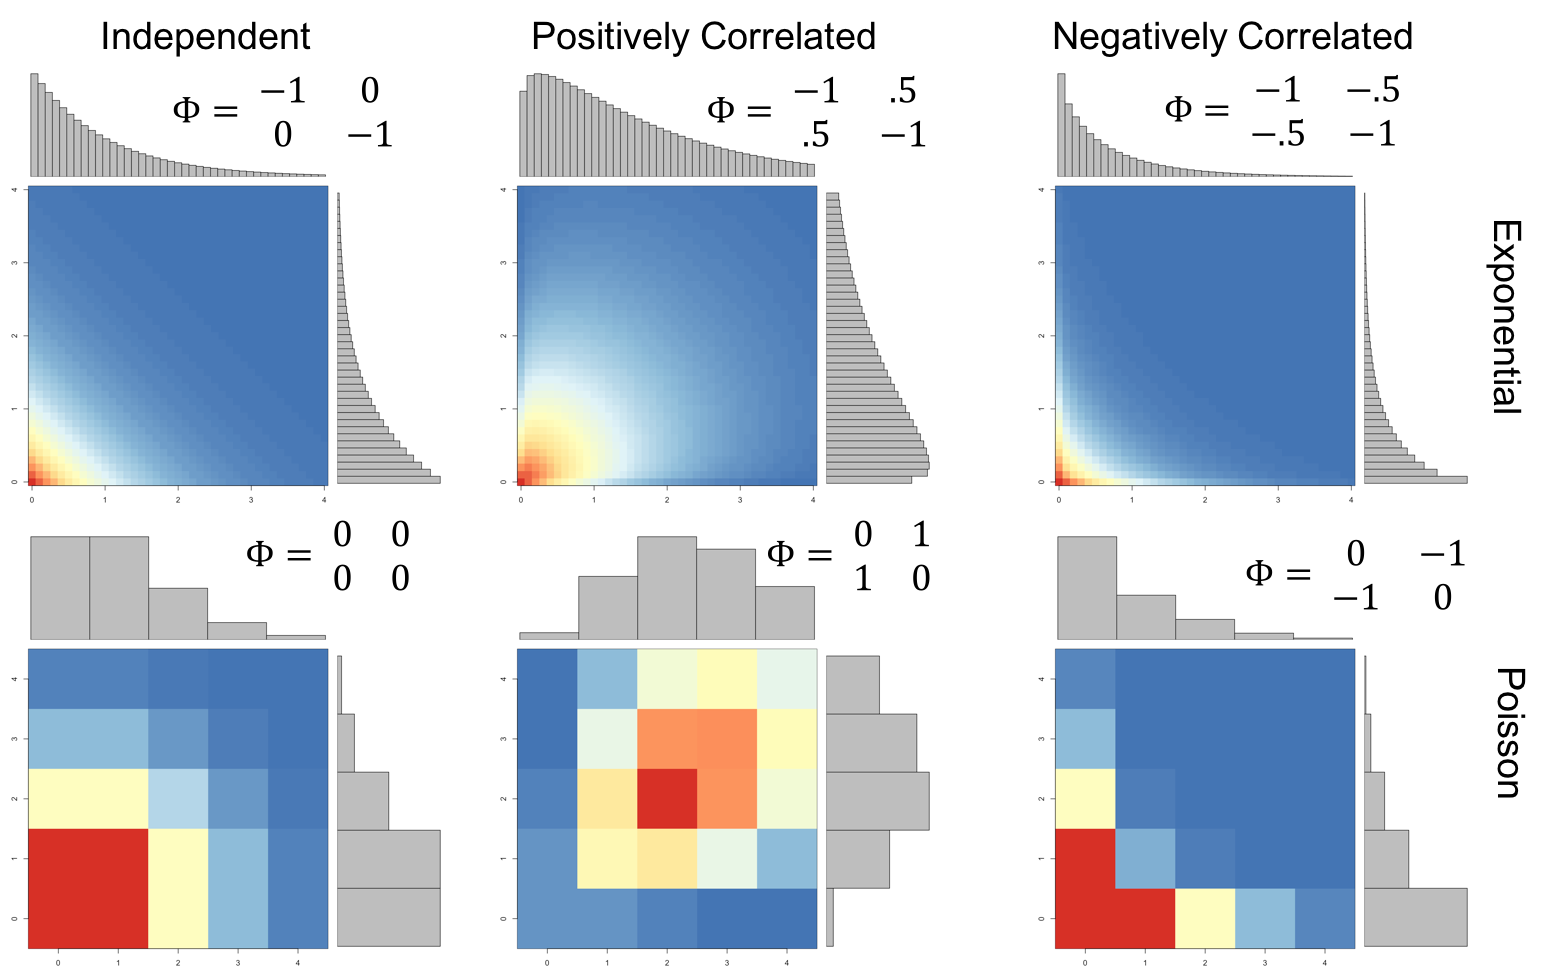
\includegraphics[width=1\textwidth]{exampledists}
\caption{Selected square root graphical model probability densities with $\Theta = \bm{0}$.  The independent parameterization of the Poisson follows from $\eta(\theta) = \log \lambda$, as in Table 1.}
\end{figure}

The proposed \textit{Square Root Graphical Model} (SRM) distribution
\[P(\bm{x} \vert \Theta, \Phi) =  \exp(\Theta^T \sqrt{T(\bm{x})} + \sqrt{T(\bm{x})}^T\Phi \sqrt{T(\bm{x})} + \sum_{s=1}^p B(x_s) - A(\Theta,\Phi))\]
enables the diagonals of $\Phi$ to be non-zero without necessitating quadratic tails.  Here, we are taking entry-wise square roots.  Non-zero diagonals of $\Phi$ enable it to be negative definite, even when off-diagonal terms are greater than zero.  While negative definiteness of $\Phi$ is sufficient for normalization, we will later show that this is not always necessary.   The SRM parameterization of the multivariate Gaussian necessitates $T_{SRM}(x) \vcentcolon = x^2$ and redefinition of the square root function $\sqrt{(\bm{x}} \vcentcolon \sgn{(\bm{x})}\sqrt{\bm{x}}$.  Under this definition, the square root and square functions are inverses, which leads to precisely the same model as in the previous section.  Some example Poisson and exponential SRM distributions are displayed in \ref{fig:exampledists}.

The diagonal terms of $\Phi$ may be considered as the scalars which completely characterize the compatibility functions associated with self-edges. Alternatively, node-conditionals as from a two-parameter exponential family.    The node conditionals of the SRM distribution are straightforward to observe by expanding the matrix multiplication. Separating terms into those which are multiplied by $\sqrt{x_s}$ and $x_s$, we see that
\[P(x_s \vert x_-s, \eta_{1s}, \eta_{2s}) = \exp{(\eta_{1s}^{node} \sqrt{x_s} + \eta_{2s}^{node} x_s + B(x_s) - A(\eta_{1s}^{node} , \eta_{2s}^{node} ))} \]
where $\eta_{1s}^{node} \vcentcolon = \Theta_s + 2 \Phi_{-s}\sqrt{x_{-si}}$ and $\eta_{2s}^{node} \vcentcolon = \Phi_{ss}$.  This distributions illustrates the useful difference of the SRM compared to the previous model:   Univariate conditionals are identical to their base exponential families in the case that $\eta_1 = 0$, and even when this is not the case, the dominating term in the node-conditional distribution is of the same order as the base exponential family.  This ensures that the node-conditionals have tail behavior which corresponds to the base distribution, alleviating a concern of previous models \citep{Yang2013-is}. Note that this is not the case in the non-square root model for any distribution with log-linear tails, and that keeping the term of largest order in the sufficient statistics, in this case $\Phi_{ss}$, at the same order as the natural parameter of the univariate node-conditional distribution exponential family distribution ensures that conditionals will be faithful to the base distribution in this sense.  In this way, square root sufficient statistics are often a natural choice pairwise graphical models.

\begin{figure}\label{fig:conditionals}
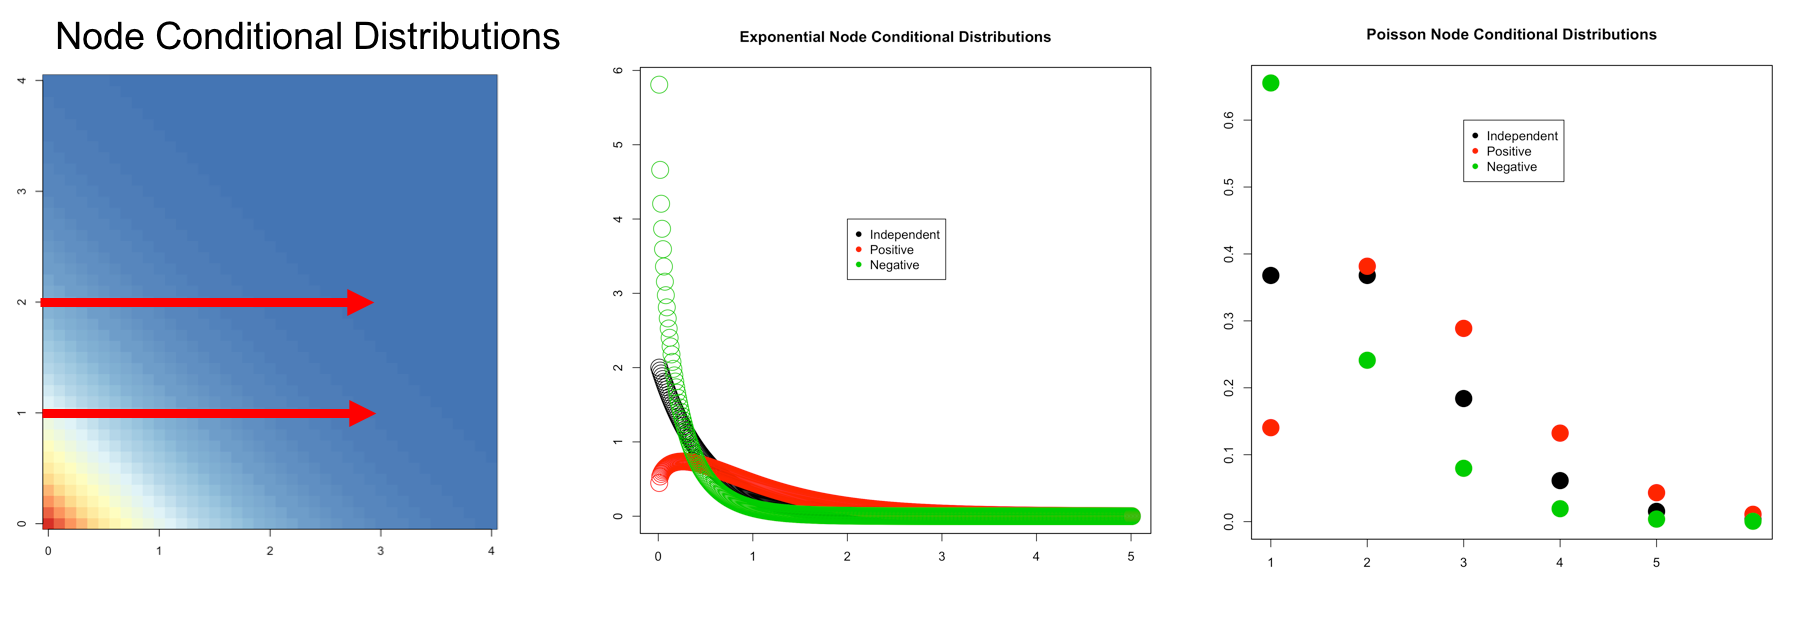
\includegraphics[width=\textwidth]{fig2condish}
\caption{The figure on the left shows selected node conditionals of a SRM bivariate exponential distribution.  The two figures on the right are the densities of exponential and Poisson node conditionals\vmadd{.} 
\vmcomment{Fonts in the plots are too small.}}
\end{figure}
\subsection{Normalizability of Square Root Graphical Models}

The SRM has a natural parameter space
\[\mathcal{N} = \{ ( \Theta, \Phi)  \vert A(\Theta, \Phi) < \infty \} , \]
where
\begin{align}
A(\Phi, \Theta) = \log \int_\mathcal{D} \exp{(\Theta^T \sqrt{T(\bm{x})} +  \sqrt{T(\bm{x})} \Phi \sqrt{T(\bm{x})} + \sum_{s=1}^p B(x_s))}d\mu (\bm{x}).
\end{align}

The natural parameter space of the SRM distribution depends on the sufficient statistics, base measures, and natural parameter spaces of the conditional probability distributions of the sites which make up the base graph.  Observe the extended normalizability of the SRM compared with the previous model by radially factorizing $A(\Theta, \Phi ) $ along $\mathcal{D}$.
\begin{align}
A(\Theta , \Phi) = \log \int_\mathcal{V} \int_{\mathcal{Z}(\mathcal{V})} \exp{(\Theta^T \sqrt{T(z \bm{v})} +  \sqrt{T(z \bm{v})} \Phi \sqrt{T(z \bm{v})} + \sum_{s=1}^p B(zv_s))} d\mu(z)d\bm{v},
\end{align}
where $\mathcal{V} =\{\frac{\vert \bm{v} \vert}{  \|\bm{v}\|_1} = 1, \bm{v} \in \mathcal{D} \}$, and $\mathcal{Z}(\mathcal{V}) = \{z \in \mathbb{R}_+ \vert z\bm{v} \in \mathcal{D} \}$.

Since $\mathcal{V}$ is bounded and $\exp$ and $\log$ are continuous, $A$ is finite as long as
 \begin{align*}
 A^{rad}(\Theta, \Phi) \vcentcolon & = \int_{\mathcal{Z}(\mathcal{V})} \Theta^T \sqrt{T(z \bm{v})} +  \sqrt{T(z \bm{v})} \Phi \sqrt{T(z \bm{v})} + \sum_{s=1}^p B(zv_s) d\mu(z)\\
 &= \int_{\mathcal{Z}(\mathcal{V})}  (\Theta^T \sqrt{\bm{v}}) \sqrt{z} +  (\sqrt{\bm{v}^T} \Phi \sqrt{\bm{v}})z  + \sum_{s=1}^p B(zv_s)d\mu(z)\\
&= \int_{\mathcal{Z}(\mathcal{V})} \eta_{1}^{rad} \sqrt{z} + \eta_{2}^{rad} z + \sum_{s=1}^p B(x_s) d\mu(z) < \infty, 
\end{align*}
where $T(x) = x$ is assumed, and $\eta_{1}^{rad} = \Theta^T \sqrt{\bm{v}}$,  $\eta_{2}^{rad} = \sqrt{\bm{v}^T} \Phi \sqrt{\bm{v}}$.  This is the case if 
 if $\eta_2 < 0$ or $\eta_2 = 0$, and $\eta_1 \leq 0$.  Note that this general condition is weaker than negative definiteness, since $\bm{v}$ is assumed to lie in the positive orthant, but nevertheless requires that the diagonals of $\Phi \leq 0$.  However, this is not required for distributions such as the SRM whose univariate conditionals have Poisson domains and tails.  This is because the Poisson base measure $B_{\textit{pois}}(x) = - \log (x!)$ is decreasing.  In particular, $\lim_{x \to \infty} \log \frac{1}{x!} < x^{-1}.$  Thus, $\Phi$ can have arbitrary positive values in the SRM-Poisson distribution, even on its diagonals.  This is important, since the natural parameter space of the Poisson distribution is $\mathbb{R}$, and otherwise we could not model a proper joint distribution of independent Poisson random variables using this method.

\subsection{Selection of Model Parameters} \label{Optimization}

The consistency of M-estimators for estimating model parameters was studied by \citet{Yang2013-wa} for the previous exponential family MRF model.  The authors assume that it is applicable throughout, and use l1-penalized proximal gradient to optimize model parameters $\Phi$ and $\Theta$ given data $\mathbb{X} \in \mathbb{R}^{n\times p}$ containing $n$ observations of $p$ variables.  As a substitute for the joint likelihood, we solve the convex penalized pseudolikelihood minimization problem
\begin{align}
 \argmin_{\Theta, \Phi} \sum_{s = 1}^{p} (-\frac{1}{n} \sum_{i = n}^n (\eta_{1si} \sqrt{x_{si}} + \eta_{2si} x_{si} - A_{node} ( \eta_{1si}, \eta_{2si} )) + \lambda\| \Phi_{s,-s} \|_1).
 \end{align}
Here, $\eta_{1si} = \Theta_s + 2 \Phi_{-s}\sqrt{x_{-si}}$ and $\eta_{2si} = \Phi_{ss}$, $i \in \{1,\dotsc, n\}$.  The optimization algorithm first proposes new values of $\Phi_{s,}$ and $\Theta_s$ which increase the likelihood.  These are identified through a series of gradient calculations.  
\begin{align*}
\frac{dO}{d\phi_{ss}} &= \frac{-1}{n} \sum_{i=1}^{n} x_{si} - \frac{dA_{node}}{d\eta_2}, \\
\frac{dO}{d\phi_{-s}} &= \frac{-2}{n} \sqrt{\mathbb{X}_{-s}}^T \sqrt{\mathbb{X}_s} - 2 \sqrt{\mathbb{X}_{-s}} \frac{dA_{node}}{d\eta_1}\, \quad \text{and}  \\
\frac{dO}{d\theta_{s}} &= \frac{-1}{n} \sum_{i=1}^{n} \sqrt{x_{si}} - \frac{dA_{node}}{d\eta_1} \\
\frac{dA_{node}}{d\eta1} &= \frac{(A_{node}((\eta_1 + \epsilon), \eta_2) - A_{node}((\eta_1 , \eta_2)))}{\epsilon} \text{and} \\
\frac{dA_{node}}{d\eta_2} &= \frac{(A_{node}(\eta_1 , \eta_2+ \epsilon) - A_{node}((\eta_1 , \eta_2)))}{\epsilon}
\end{align*}
In general, $A_{node}$ is easy to approximate since it is an integral over only one dimension. However, in the case that univariate conditionals are, exponential it has the analytic solution
\[A_{node} (\eta_1, \eta_2) = \sqrt{\pi}  \eta_1 \frac{\exp{ ( \frac{\eta_1^2}{-4\eta_2} ) }} { (2(-\eta_2)^{1.5})} (1 - \erf{(\frac{-\eta_1}{2 \sqrt{ -\eta_2}}}))  + \frac{1}{-\eta_2}.\]
The authors suggest $\epsilon = 0.0001$.
After the off-diagonal values of each proposed $\Phi$ are soft-thresholded using the proximal operator $ST(\Phi_{off}) = \sgn{ (\Phi_{s,-s} )} (\Phi_{s,-s} - \lambda)_+$, the penalized univariate-conditional probability of the move is computed, and significant improvements are accepted.  After each computation of the gradient, large jumps are proposed, and if these are rejected, smaller jumps are considered.  Note that parallelization of the minimization problem eliminates a computationally intractable application of the chain rule, and generates two estimates of every off-diagonal element of $\Phi$, of which we take the average.

\subsection{Estimation of Normalization Constant}
We use the MCMC algorithm Annealed Importance Sampling to estimate the normalizing constant $A(\Theta, \Phi)$ of the fitted SRM.  Standard importance sampling enables estimation of the area under a function by a number of comparisons of its density with the density of another functions whose normalizing constant is known.   Annealed importance sampling is the repeated application of this principle.  In our case, this comparison is made over a sequence of intermediate densities
\[P_i(\bm{x} \vert \Theta_i, \Phi_i) =  \exp(\Theta_i^T \sqrt{T(\bm{x})} + \sqrt{T(\bm{x})}^T\Phi_i \sqrt{T(\bm{x})} + \sum_{s=1}^p B(x_s)) \]
where $\Phi_i = \Phi_{diag} + \frac{i}{n} (\Phi - \Phi_{diag}),$ and $\Theta_i = \frac{i}{n}{\Theta}$ for $i \in 0, \dotsc n$.  

The usefulness of AIS stems from the limited differences between each distribution iterate.  Subsequent distributions can be sampled from efficiently using MCMC based upon the previous iterate.  That is, each for each point $x_i$ in a particle path $x = \{x_0, \dotsc x_n\}$, a series of Metropolis-Hastings of Gibbs sampling moves are used to ensure that each of our particle paths is remaining in a region of high density.  Since we expect the differences between successive distributions to be small, this does not require very many moves.  We then compute the product of the importance weights $w(x) = \prod_{i=1}^n \frac{f_{i-1}(x_{i-1})}{f_{i}(x_{i-1})}$.  The average of these particle path weights converges to the ratio of the normalizing constants of $P_0$ and $P_n$.  Since $P_0$ is simply a probability law composed of the product of independent exponential family distributions, its normalizing constant $A_0$ is the sum of the normalizing constants of the independent univariate exponential family distributions with parameters given by the diagonals of $\Phi$.  We can therefore solve
\begin{align}
A(\Theta,\Phi) = A_0 - \frac{1}{n} \sum_{j=1}^{J} w(x_j)
\end{align}
where $J$ is the total number of particle paths.  



 \section{Results} 
 
 To illustrate the use of the SRM model, particularly its ability to model positive dependencies, we apply it to a dataset comprised of the average plane delay times on each day at 2014's 30 busiest US airports.  The delay time of all $p = 30$ airports is a random vector $\bm{x} \in \mathbb{R}^{30}$ which we observe $n=365$ times.  We instantiate an exponential SRM joint distribution with the exponential sufficient statistic $T(x) = x$ and exponential base measure $B(x) = 0$ and set the diagonals of $\Phi$ equal to maximum likelihood estimates of independent exponential distributions, i.e. the negative mean delay times.  $\Theta = \bm{0}$ and the off-diagonal elements of $\Phi = \bm{0}$.  We then use the proximal gradient descent method described in section 3.6 to optimize $\Phi$ and $\Theta$.  
 
 \begin{figure}\label{fig:map}
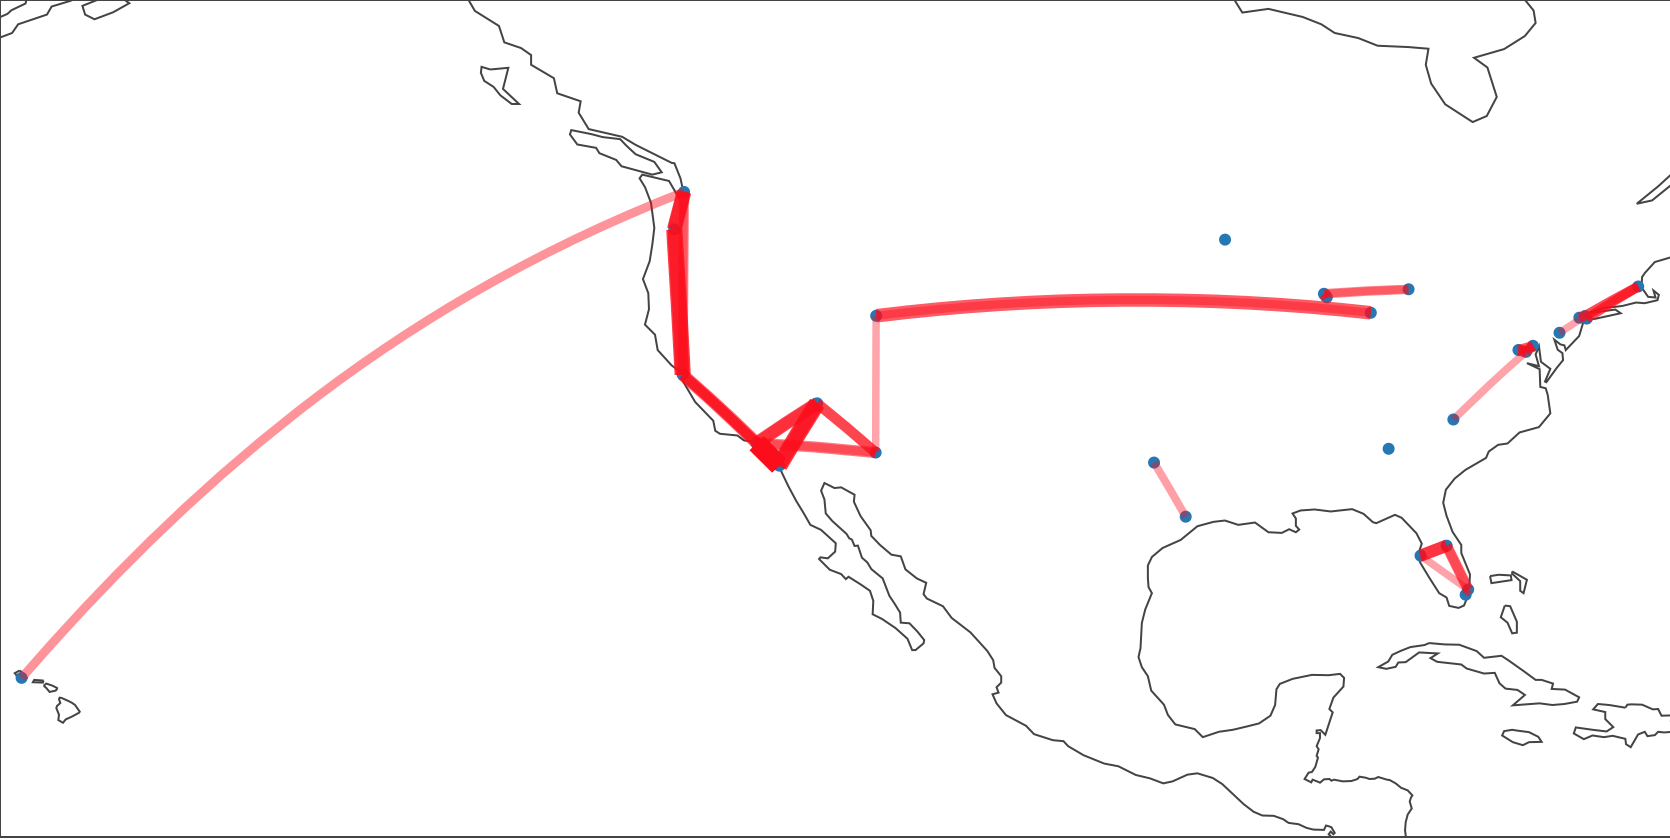
\includegraphics[width=\textwidth]{map}
\caption{Replication of the airport delay time analysis of \citep{Inouye}.  The 50 largest non-diagonal entries in $\Phi$ are displayed. While the 50 largest edges in magnitude are all positive, several smaller negative edges are present after the 50th. }
\end{figure}

Despite slight differences such as the absence of negative associations from my top 50 edges, the recovered map is very similar to the one reported by \citep{Inouye2016-hl}.  That the displayed conditional probability dependencies are all positive shows that the previous model of \citep{Yang}, which did not allow for positive dependencies, is insufficient for this data set.  A latent location factor may appear in Florida and the North East.  This makes sense given the importance of weather to on-time performance.  However, the broadly correlated delay times of the West Coast are probably not weather related.  Another candidate for causing this network are cascading delay times between long Western flights. We also might expect that the hubs of a certain airline would be correlated for this reason.  The general trend towards positive correlations is expected given that latent factors which increase delay times such weather or cascading delays tend to be shared between airports. This initial result was acquired using $\lambda = 0.0000464$ selected by the authors using cross validation.

 \begin{figure}\label{fig:likelihoods}
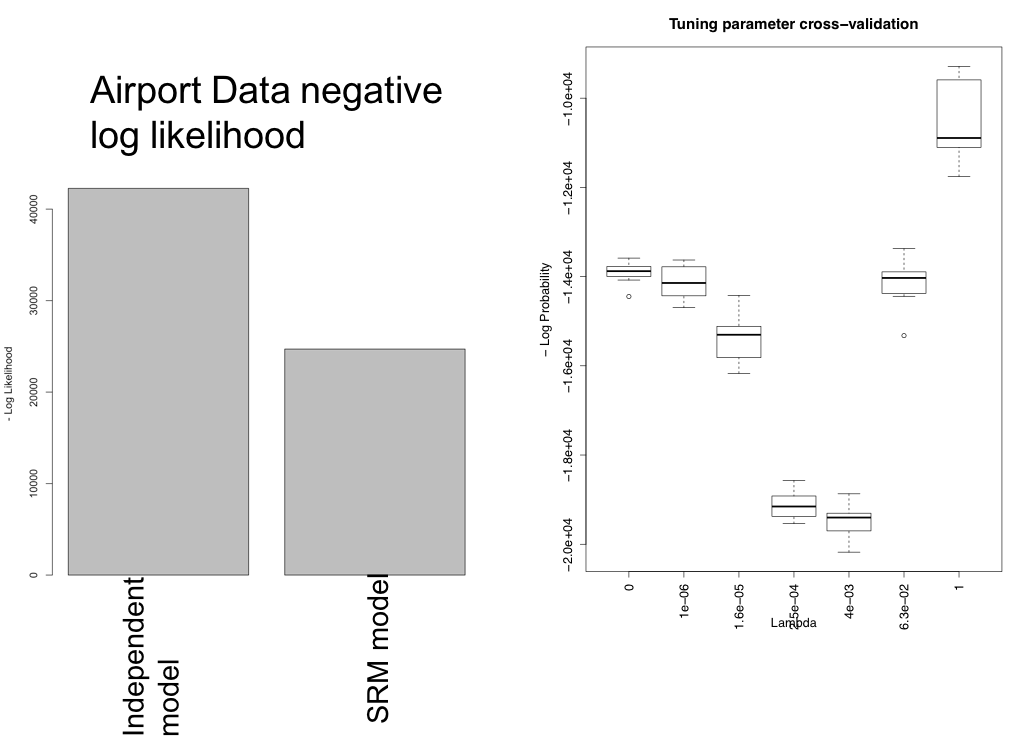
\includegraphics[width=\textwidth]{likelihoods}
\caption{On the left is a replication of the model likelihood of the independent exponential and fitted SRM models for the airport data set.  On the right are the results of cross-validations containing 10 random permutations of 50 percent of the data over a range of lambda values.}
\end{figure}

The fitted SRM model improves has a higher likelihood than the model in which each airport's delay times at independent exponential distributions with rate determined by the MLE (this independent model is the same as $P_0$ from the sampling procedure.  Note that in the preliminary Arxiv version, the authors reported an incorrectly high likelihood of the SRM model.  They now report a negative log likelihood of 23576, which very similar to the 24705 that I got. I verified the effectiveness of my sampler by adapting it to integrate multivariate Gaussians, whose normalizing constant may be explicitly computed.  I used 2000 particles, 200 intermediate distributions, and 20 Metropolis-Hastings steps per jump between intermediate distributions, but these values seemed higher than necessary, and I reduced them for cross-validation.  To verify the authors' choice of tuning parameter, I also performed a cross-validation study by training the SRM model on 10 random samples of 50 percent of days at a range of lambdas, and computed the likelihood of the models given each 50 percent of the held-out data.  Note that the 10 percent held out data size used by the authors may be especially problematic given seasonal variations in delay correlations.  These results support a small choice of $\lambda$ such as the one that I used, but also illustrate that when correlations are in general positive, conditional probability dependencies may be summarized in the $\Theta$ term.   This would probably not be the case for variables with richer positive and negative dependencies, but a model which fixes $\Theta = \bm{0}$ may be preferable for a variety of reasons.

 \section{Discussion}
 
Here, we have shown that including square roots in multivariate models is useful for controlling tail behavior in multivariate distributions.  Note that control of tail behavior is high related to the ability to specify normalizable models via negative definiteness of the interaction matrix $\Phi$.    Specifying tail distributions through the diagonals of $\Phi$ ensures that these terms are asymptotically dominant.  Non-zero diagonals of $\Phi$ enable this matrix to be negative definite, even when other elements of $\Phi$ are greater than zero.  In the Poisson case, this restriction is relaxed even further by the asymptotic decrease of the Poisson base measure.  Given the plethora of exponential family distribution with sufficient statistics in $o(x)$, square root sufficient statistics may be a natural choice for pairwise graphical models.  

The standard multivariate exponential and Poisson distributions are connected to the multivariate Gaussian through a series of limit theorems.  Understanding these limit theorems in the context of models such as this one with is interesting.  For example, diagonal elements of the SRM-Poisson interaction matrix $\Phi$ are the logs of the independent rates, but the off-diagonal elements do not have an intuitive interpretation.  
It is important to note that both node and conditional distributions are not from the base exponential family, but rather are two parameter exponential family distributions with sufficient statistics given by $T(x) = \{ \sqrt{x}, x \}$.  Obviously, tail behavior is dominated by the term that is $o(x)$, but the square root term affords a type of distributional control not present in the base distribution.  While this may be desirable, distributions of this form are certainly not as well studied as their base families.

An interesting modification to the SRM is to set $\Theta = \bm{0}$.  This restriction precludes instantiation of a multivariate Gaussian with non-zero mean, but we have tacitly acknowledged through our choice of Gaussian sufficient statistic in the SRM model, $T(x) = x^2$ and redefinition of the square root operator that in fact the model of \citep{Yang} was the natural parameterization for this distribution.  In the exponential and Poisson cases, a natural parameterization with marginals from the base distribution is not obvious.   In these cases, there is certainly no restriction for the Hammersley-Clifford based multivariate exponential and Poisson distributions to have a non-zero $\Theta$ term, and indeed non-zero $\Theta$'s may allow deviation from the base distribution to an unnecessary extent.  By eliminating $\Theta$, all deviations from the base exponential family term will depend on conditional probabilities.

This modification may be considered in parallel to the constraints on moments and domains under which SRM distributions are maximum entropy.  While a positive $\Theta$ does not effect domain or tail behavior, it certainly effects moments.  Independent distributions which are univariately maximum entropy have radial conditionals that are maximum entropy under the same constraints, as long as $\Theta = 0$. Square root sufficient statistics can be natural for pairwise graphical models, but leads to different distributions than latent variables models such as the multivariate exponential and Poisson.  Comparing the constraints under which these classical models are maximum entropy with the constraints of the SRM model could aid in interpreting this distribution. 

Within the restrictions shown by \citep{Besag1974-qb} and \citep{Yang2013-wa}, we may consider diagonal terms of $\Phi$ to correspond either to self-edges in the graphical model, or a second sufficient statistic in each univariate conditional which is the square of the first.  Both these characterizations have weaknesses.  In the first case, self-edges are somewhat difficult to interpret as conditional probabilities.  Furthermore, the presence of self-edges suggests that n-roots of sufficient statistics may be composed on the diagonals of n-way tensor products in graphical models with cliques of size greater than 2.  In this interpretation, diagonals correspond to trivial self-cliques n-simplices, and interactions may in fact be considered using combinations of n-th roots, with out violating the theorem of \citep{Besag} and \citep{Yang}.  In the second case, one term of the corresponding natural parameter pair frequently needs to be zero.  It seems that these characterizations are somewhat interchangeable. 

While MRF decompositions have guaranteed consistent neighborhood recovery and learning of graph structure, the exact applicability existing estimation schemes this particular model has not been verified.   The square rooting of sufficient statistics seems as though it may alter the convergence rates of neighborhood recovery and confidence intervals.  Airport delay times are not i.i.d.  For example, delays may be worse in winter.  I attempted to mitigate this concern somewhat by utilizing large samples for cross-validation,  but this unfortunately contradicts as central assumption in the previous characterization of our estimator \citep{yang}.  However, given the large array of methods for univariate model fitting, it seems likely that there are many promising areas for addressing this concern.

As an alternative to joint likelihood-based model selection, a strategy which assess model fit non-parametrically or only on univariate conditionals may be used.  These avoid computation of the troublesome normalizing constant.  Interestingly, in certain cases from math and physics, there exist tractable ways of deriving this constant from subtle properties of the base graph.   While pleasingly general analytic solutions for this constant seem somewhat hopeless given the large number of potential cliques in a high-dimensional graph, these methods may help us to understand the trade off between complexity of a MRF's graph structure, and the complexity of its univariate conditionals.

Finally, note that since exponential families are the only distributions which have sufficient statistics of fixed size, distributions outside this class are less amenable to multivariate generalizations, since the number of terms governing the interactions between these statistics can grow with the data.  In this way, univariate exponential families are appealing as univariate conditionals of multivariate probability measures.  That these univariate families are multiparameter distributions of a potentially novel nature is necessitated by the conditions of an MRF.
 
 \vmcomment{Clean up your references and don't forget to protect your capitalization, e.g., Poisson, not poisson.}
 
  \bibliography{samkoelleprelimworking}
   \end{document}